\documentclass[16pt,latin]{scrartcl}
\usepackage[utf8]{inputenc}
\usepackage[T1]{fontenc}
\usepackage[paperheight=297cm,paperwidth=210cm, left=1mm,right=1mm,top=1mm,bottom=1mm]{geometry}
\usepackage{babel}
\usepackage{microtype}
\usepackage{graphicx}
\usepackage{xcolor}
\usepackage{blindtext}
\usepackage{tikz}
\usepackage{mdframed}
\usepackage[]{tcolorbox}
\usepackage{eso-pic}
 
\setlength{\parskip}{0pt}
\setlength{\parindent}{0pt}
\pagestyle{empty}
 
\begin{document}
 
\begin{center}
{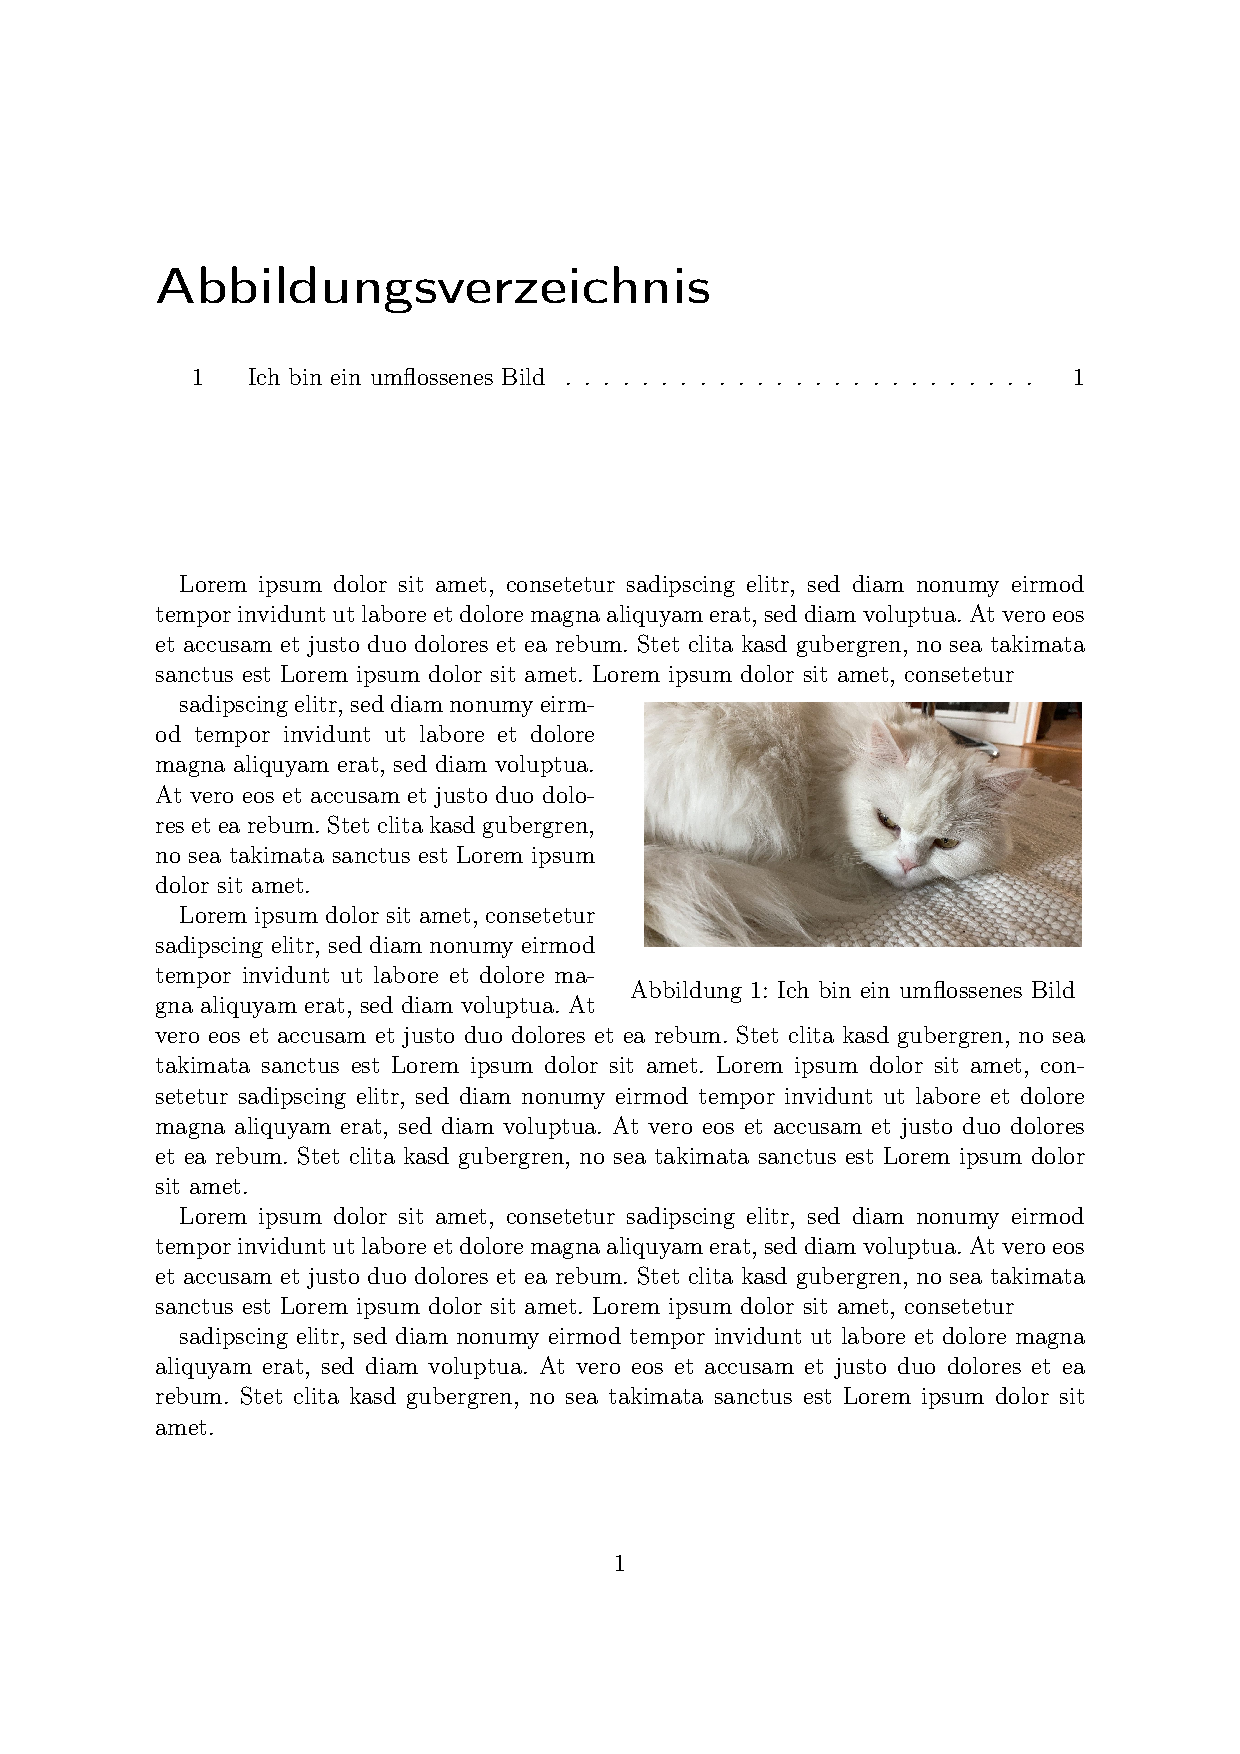
\includegraphics[width=\linewidth]{Bild-umfliessen.pdf}}
\end{center}
 
 \AddToShipoutPictureFG{
  \put(1100,4050){
{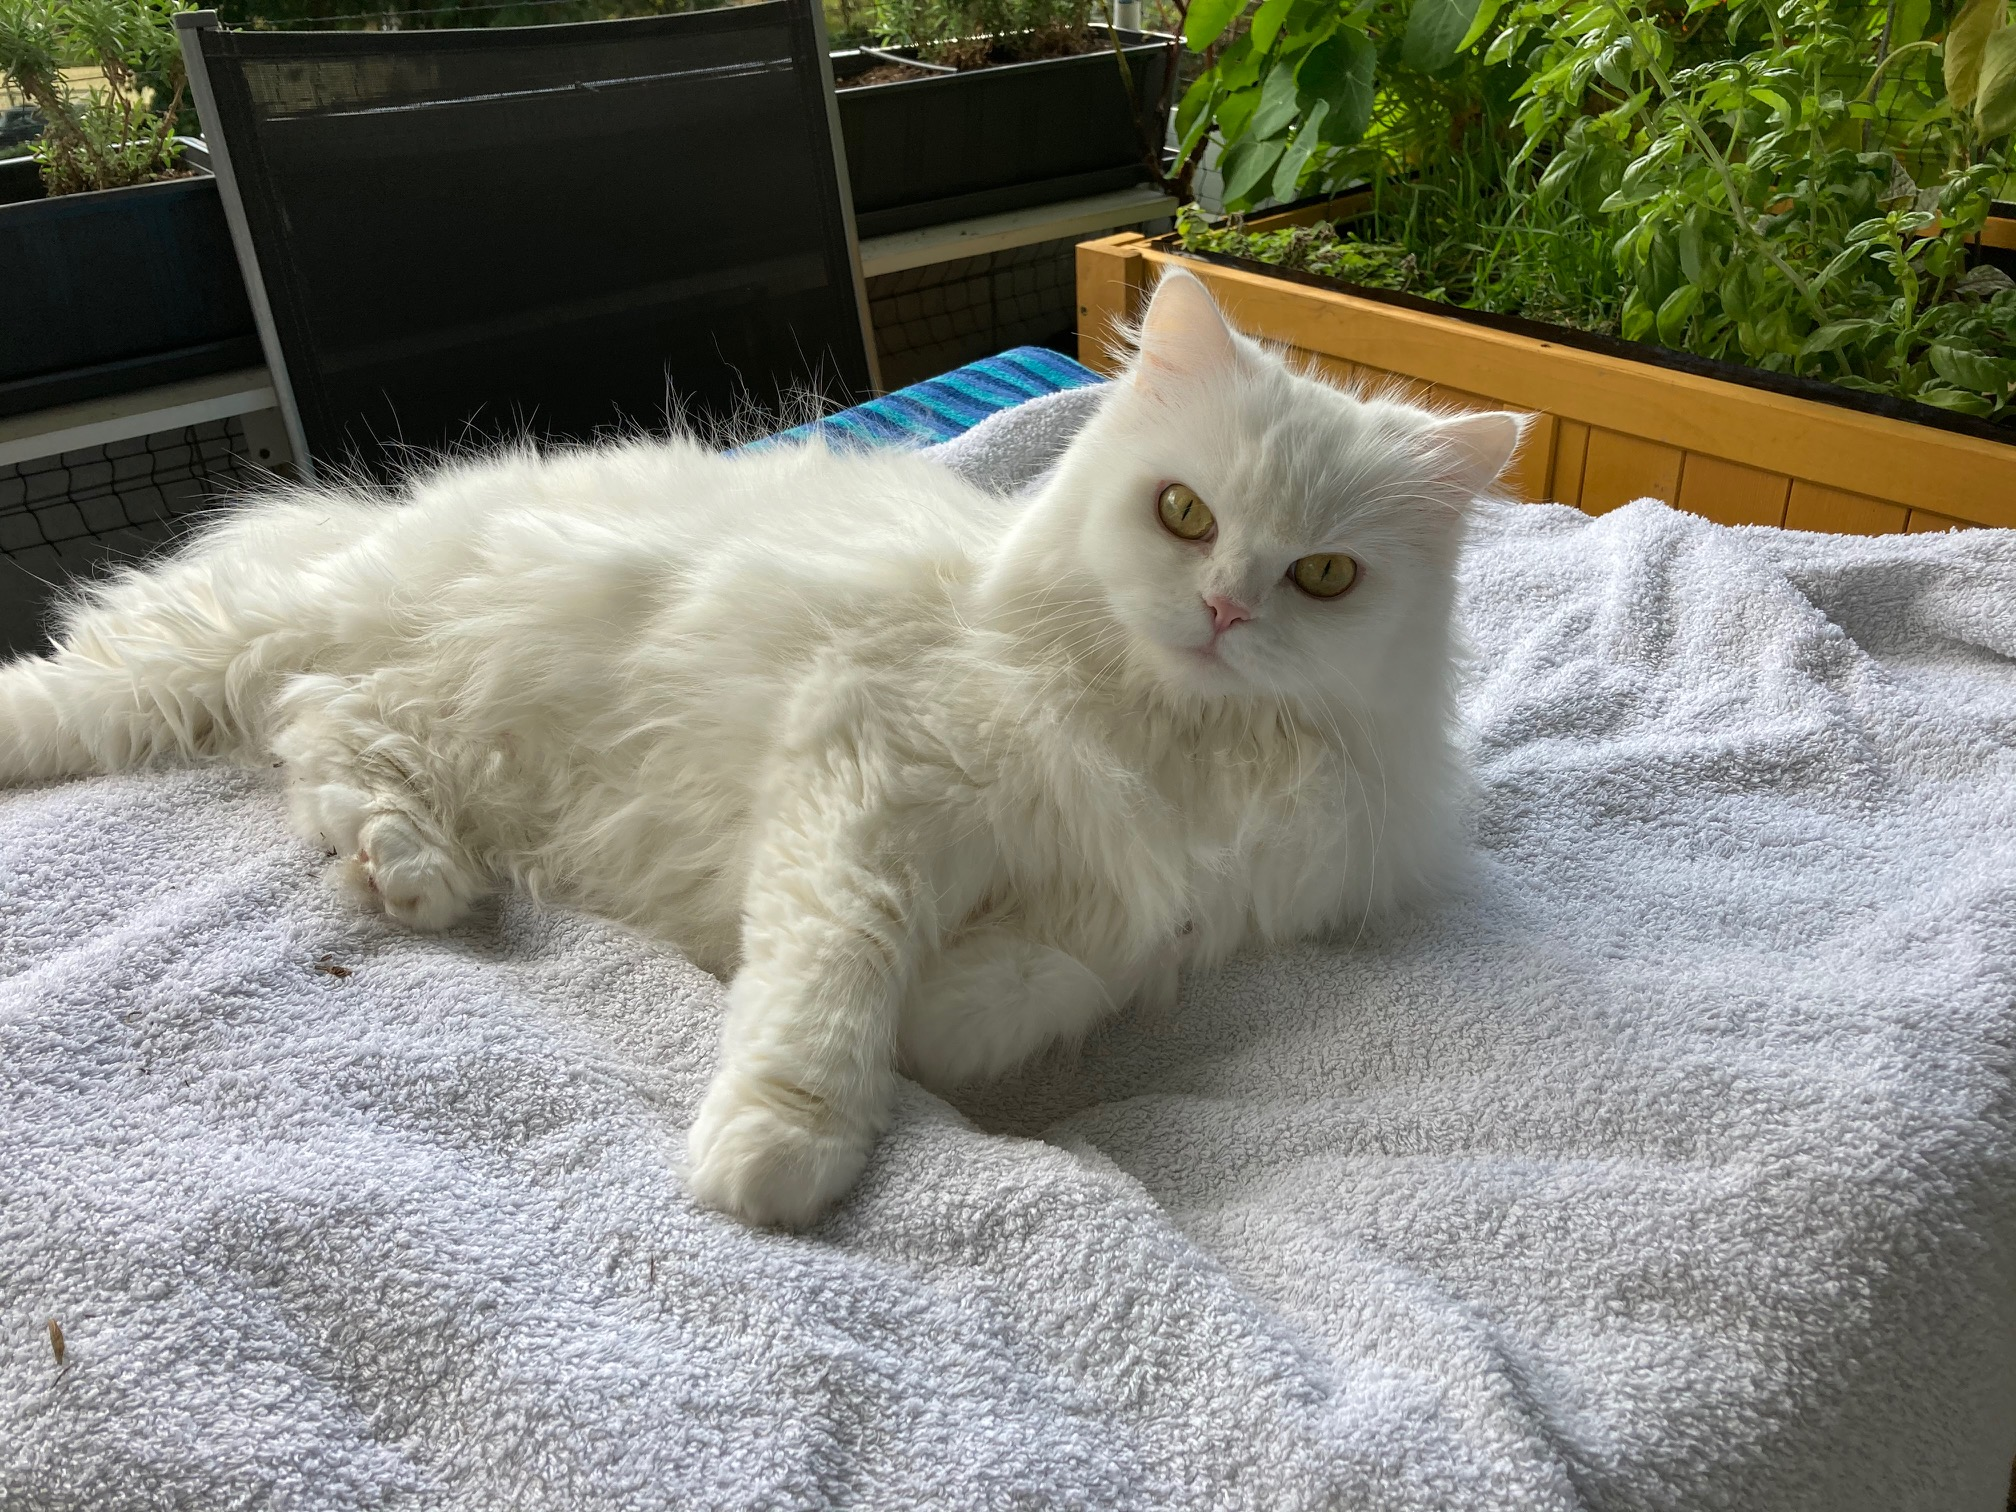
\includegraphics[width=0.5\textwidth]{./Bilder/Katze1.jpg}}
}}
 
\AddToShipoutPictureFG{
  \put(200,1050){
  \scalebox{1.5}{%
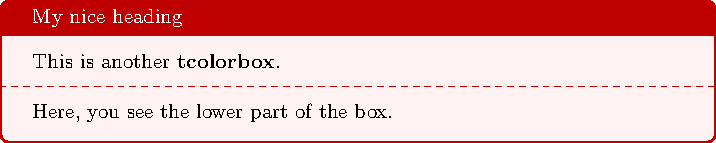
\includegraphics[width=0.5\textwidth]{stand-01}
}}}
 
 
\end{document}



 \begin{tcolorbox}[colback=red!5!white,colframe=red!75!black,title=My nice heading]
This is another \textbf{tcolorbox}.
\tcblower
Here, you see the lower part of the box.
\end{tcolorbox}
 

 

 
\AddToShipoutPictureFG{
  \put(1100,4050){
\colorbox{gray}{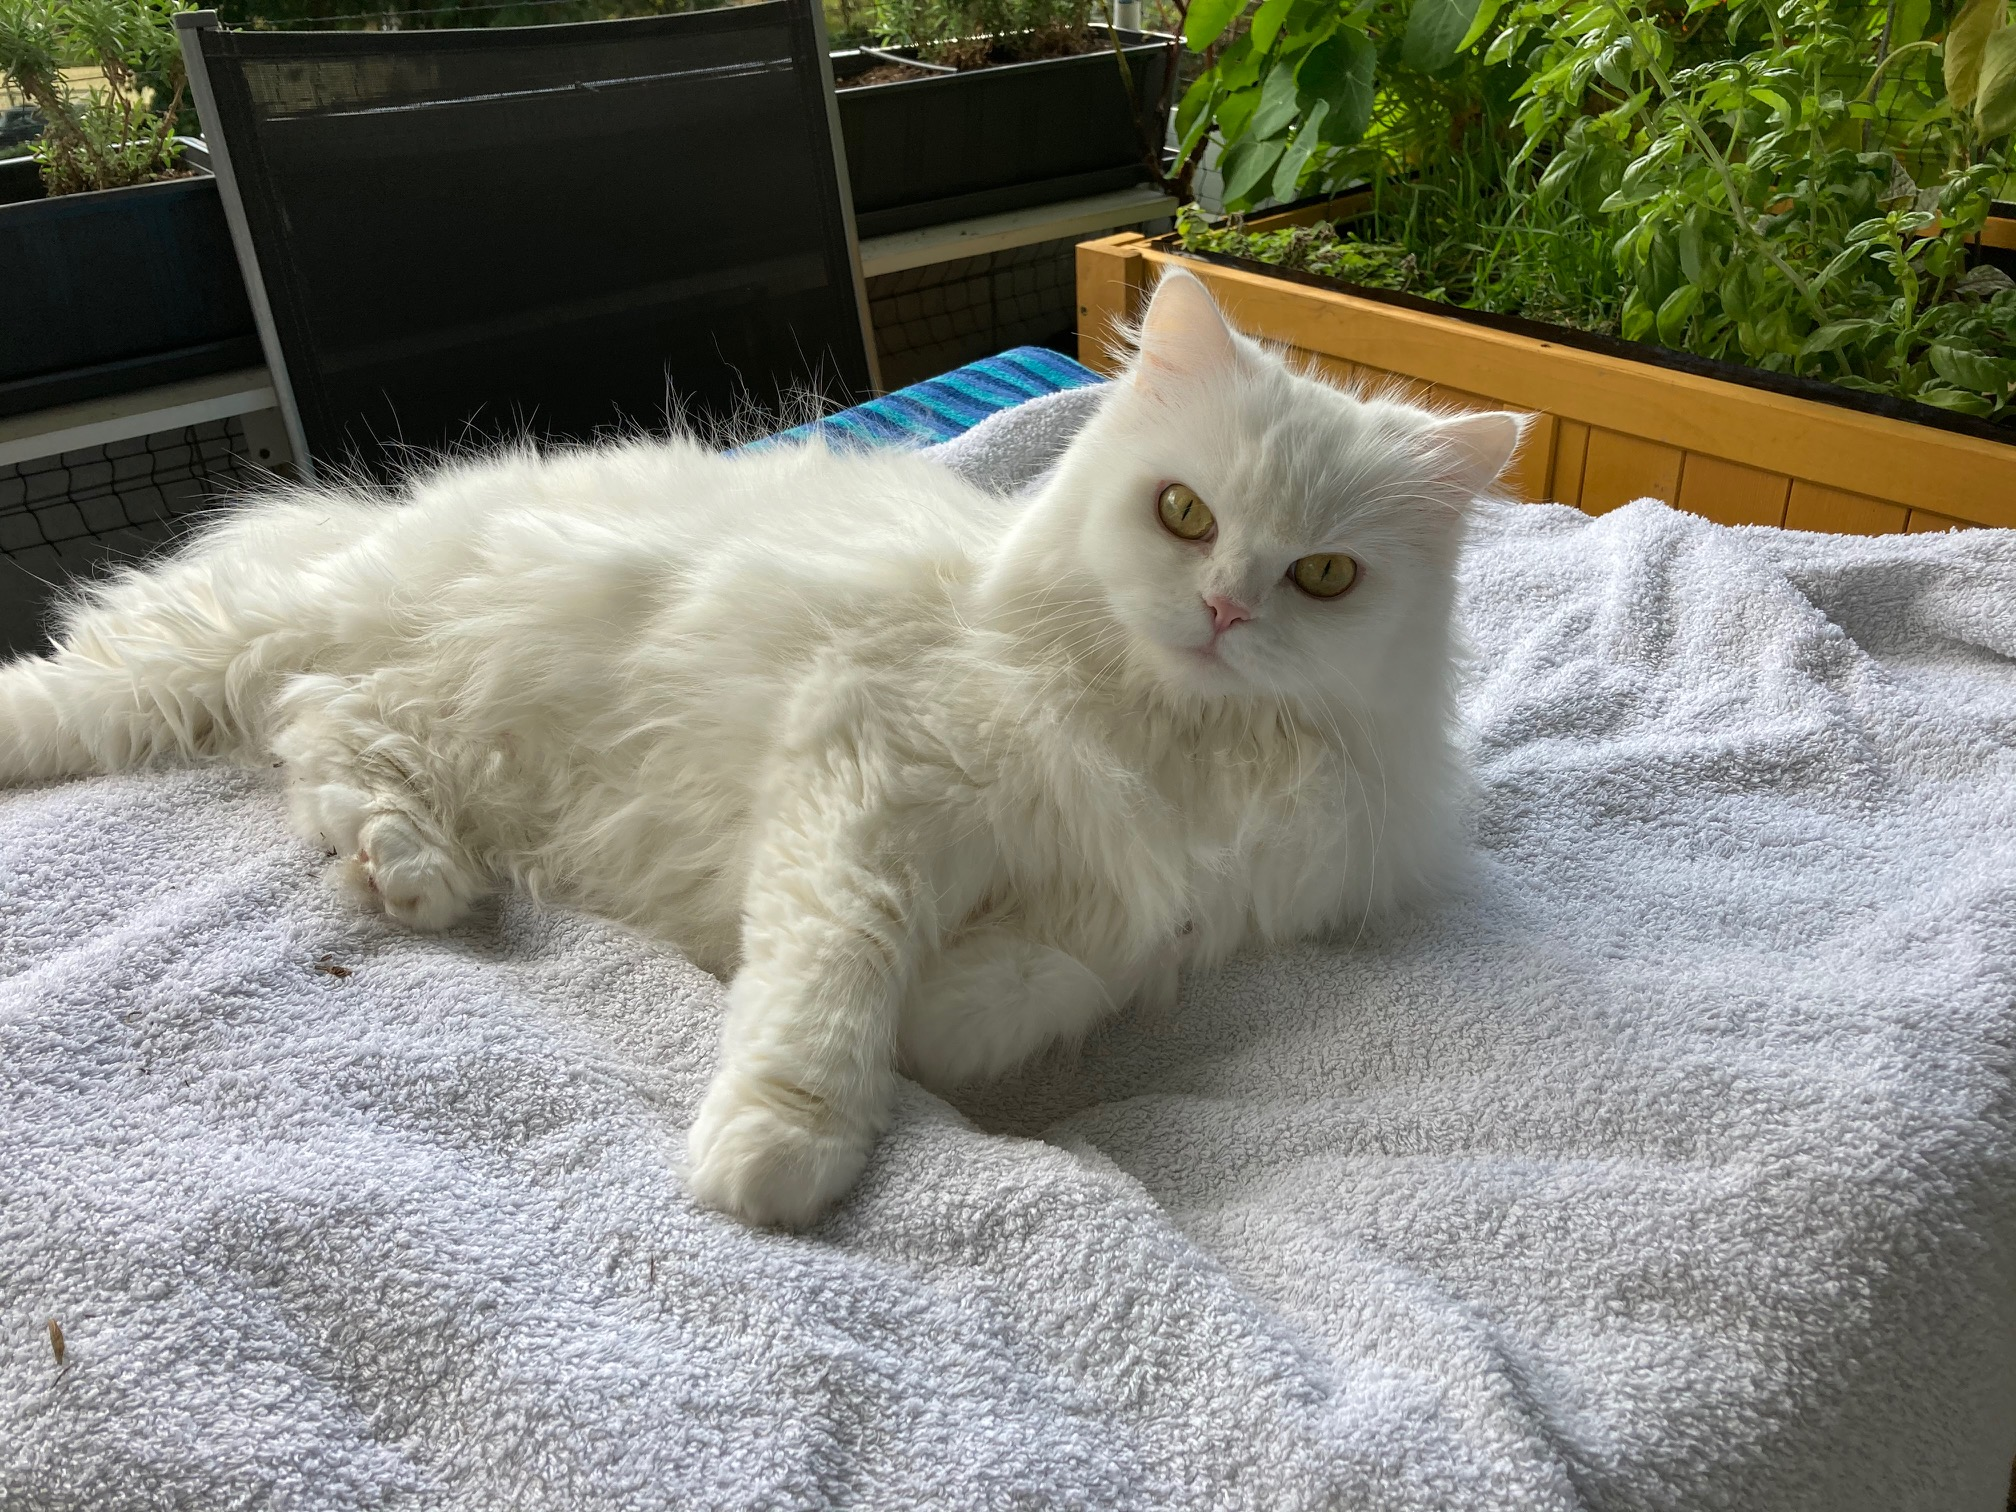
\includegraphics[width=0.5\textwidth]{./Bilder/Katze1.jpg}}
}}
 
\AddToShipoutPictureFG{
  \put(100,3450){
\colorbox{gray}{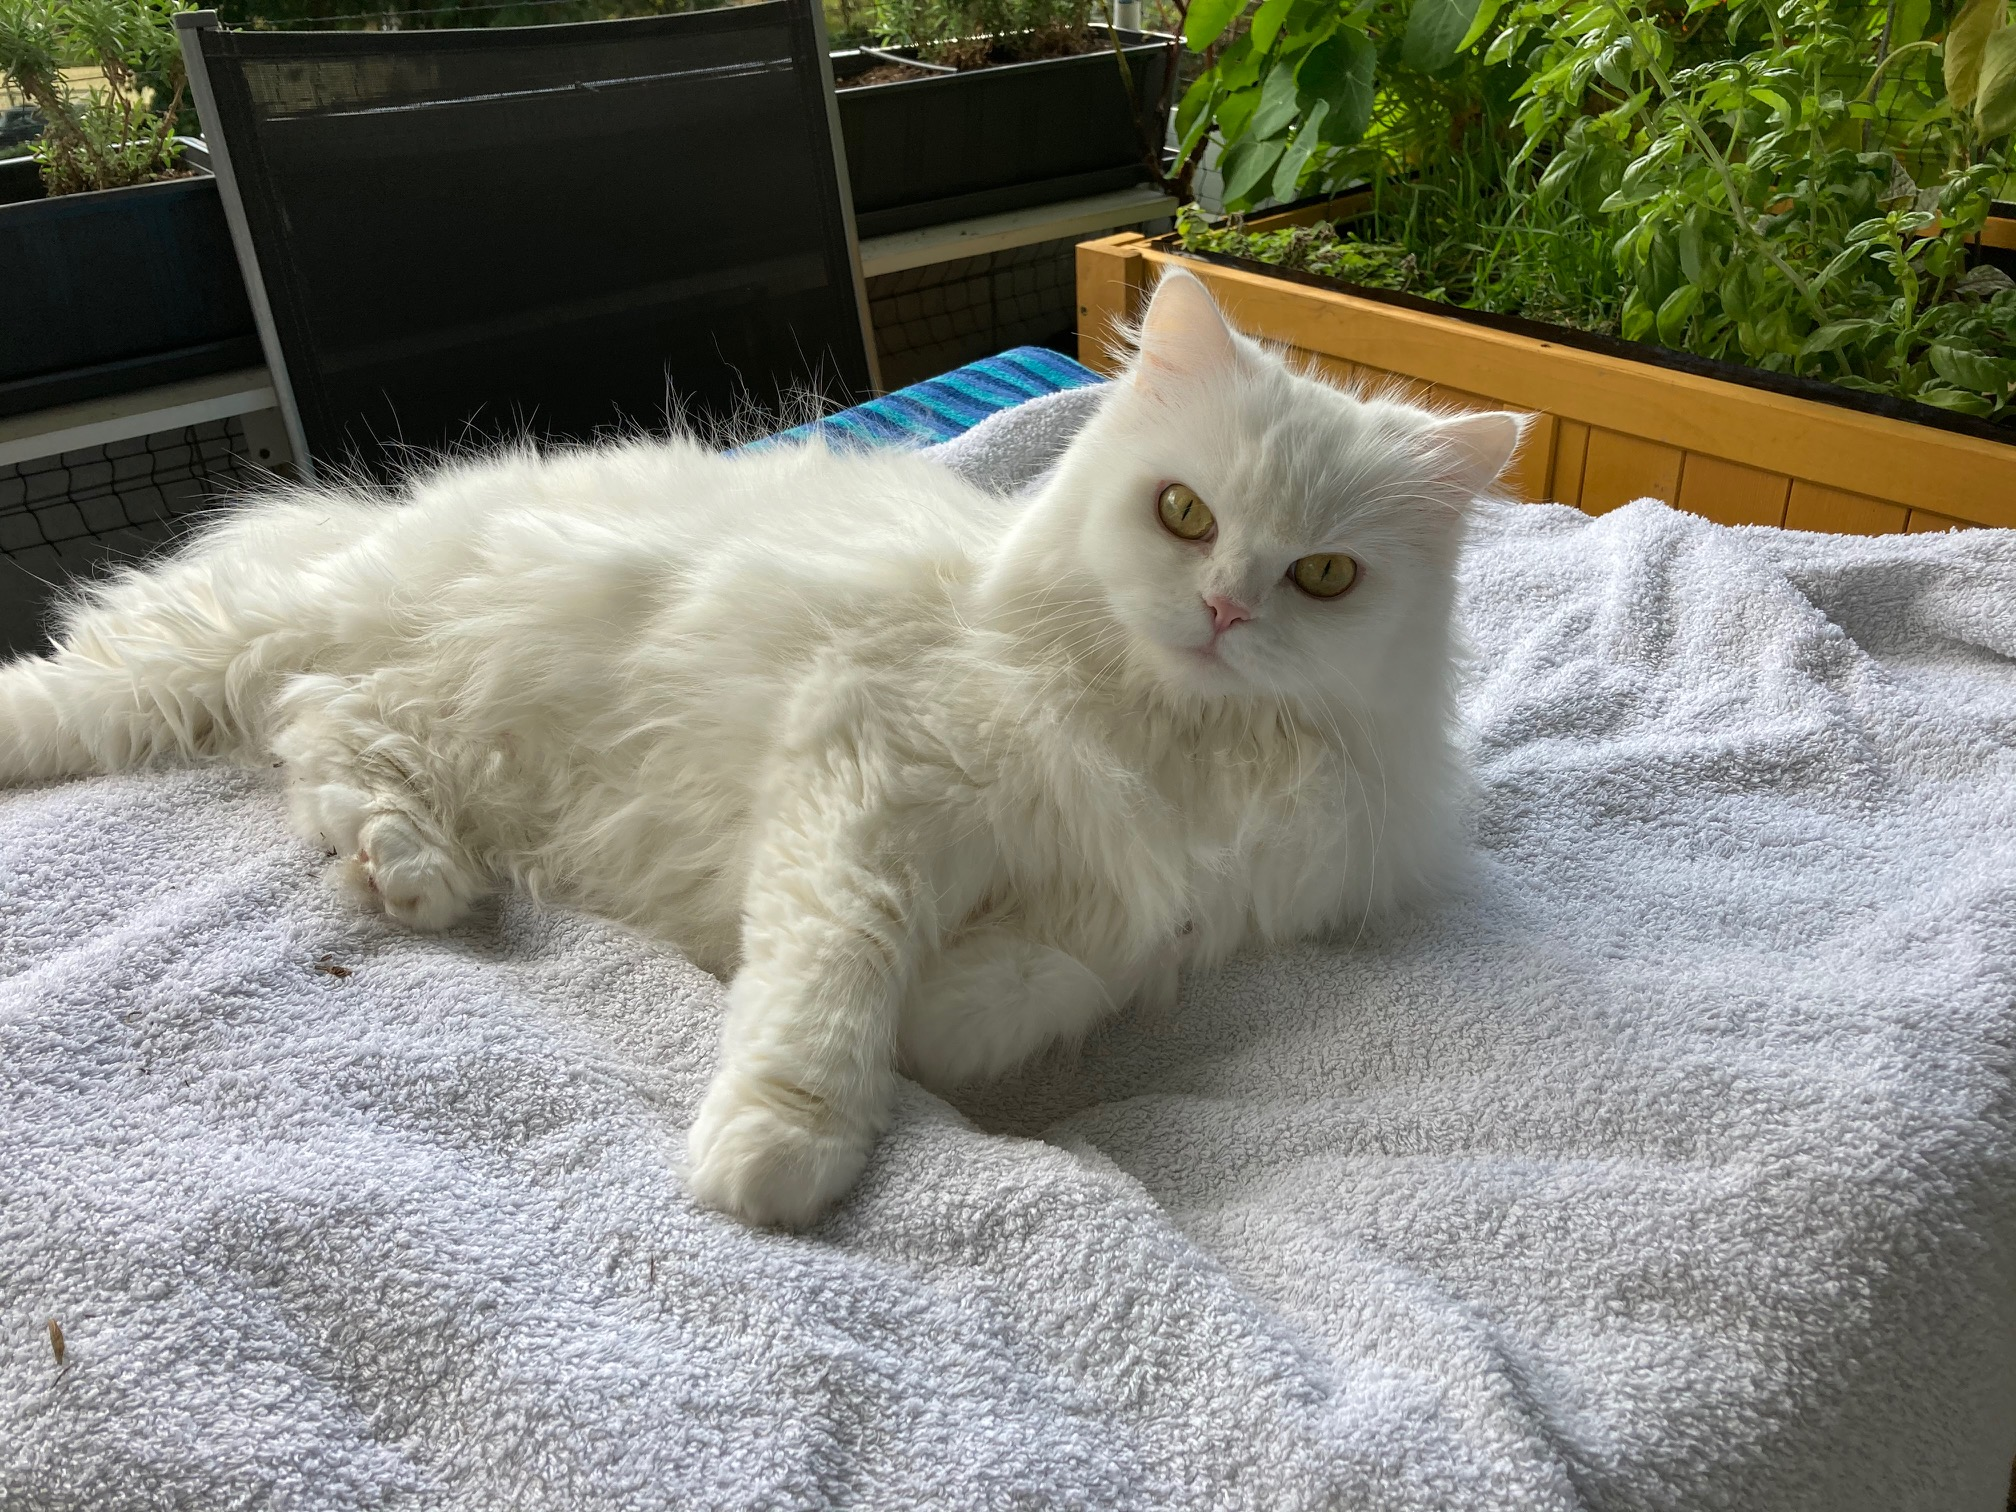
\includegraphics[width=0.5\textwidth]{./Bilder/Katze1.jpg}}
}}
 
\AddToShipoutPictureFG{
  \put(1100,3000){
\colorbox{gray}{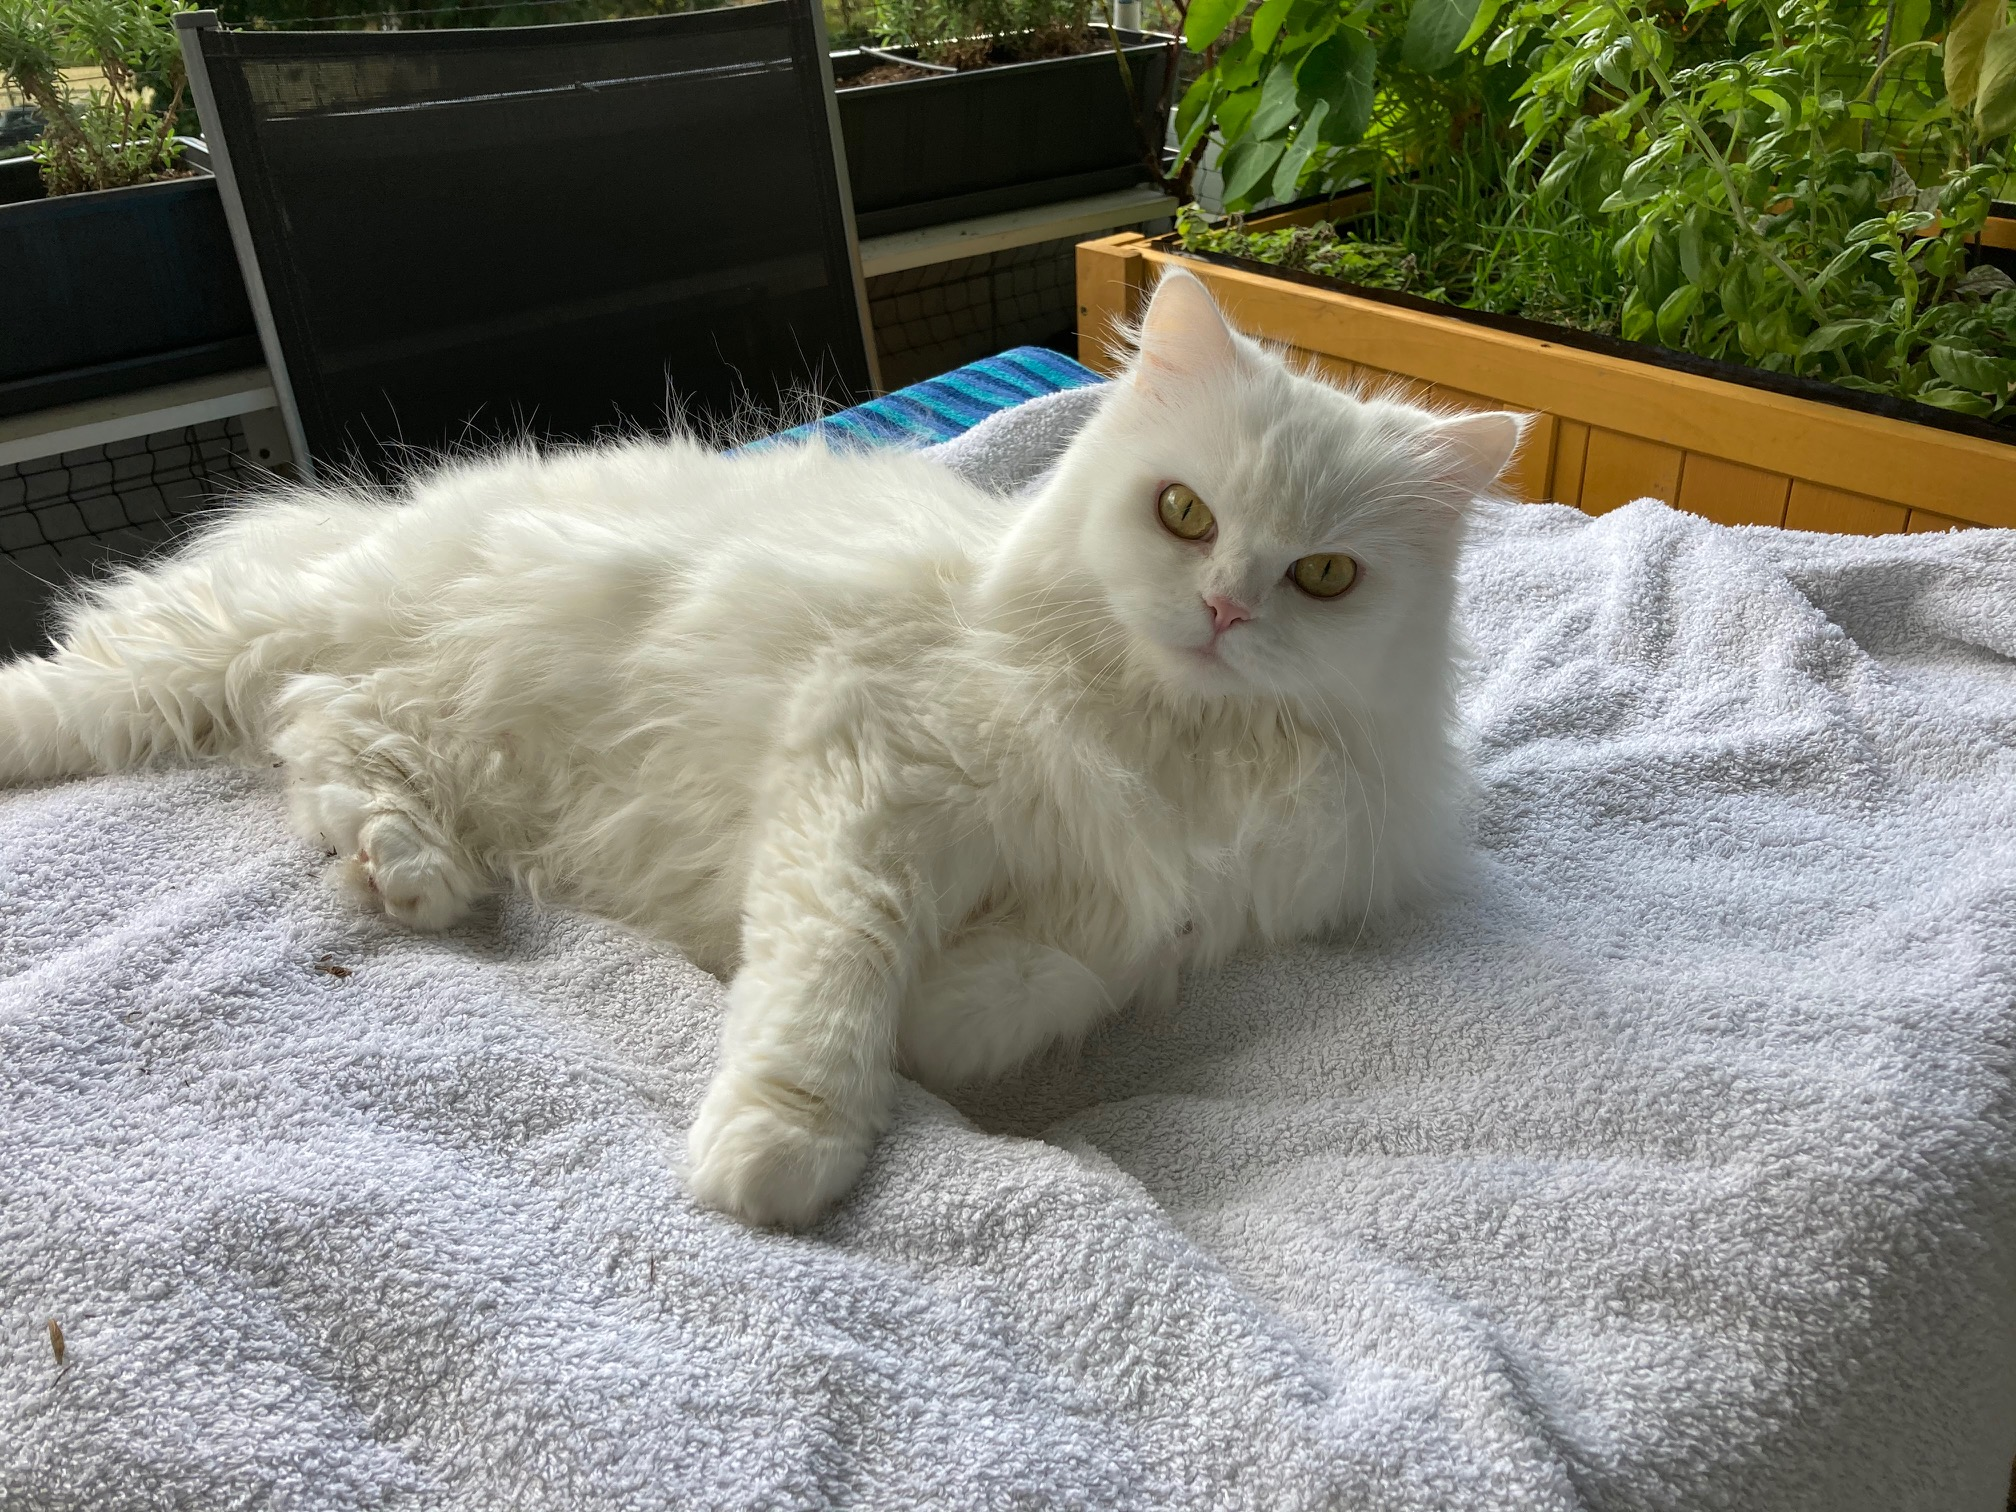
\includegraphics[width=0.5\textwidth]{./Bilder/Katze1.jpg}}
}}
 
 
 
\AddToShipoutPictureFG{
  \put(100,2290){
\colorbox{gray}{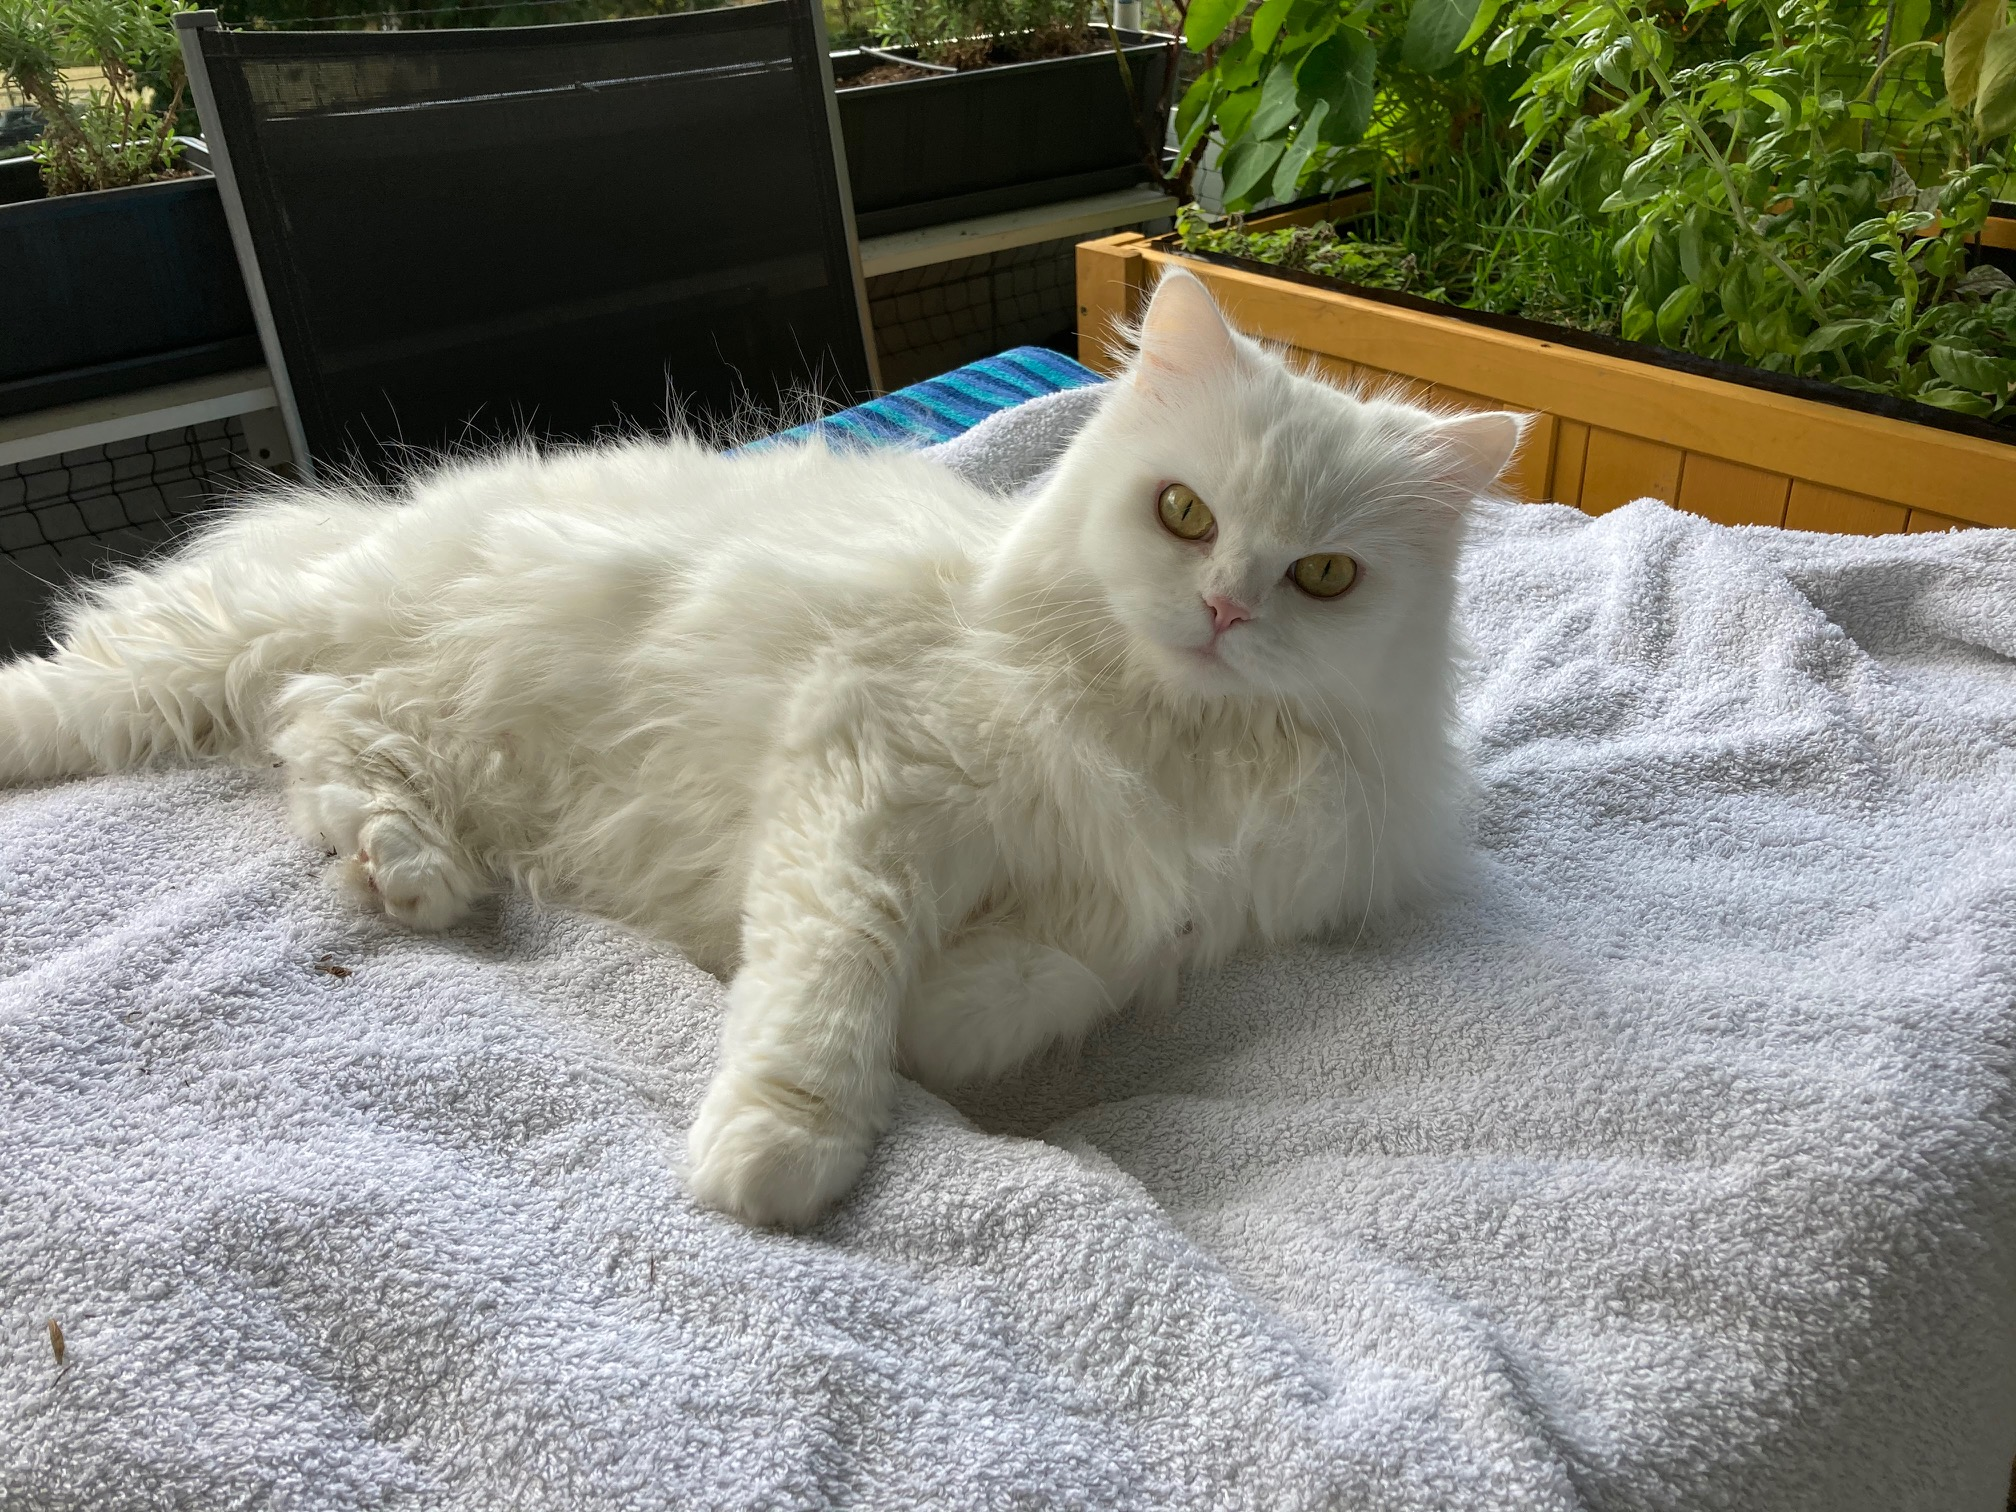
\includegraphics[width=0.5\textwidth]{./Bilder/Katze1.jpg}}
}}
 
 
\AddToShipoutPictureFG{
  \put(1100,1950){
\colorbox{gray}{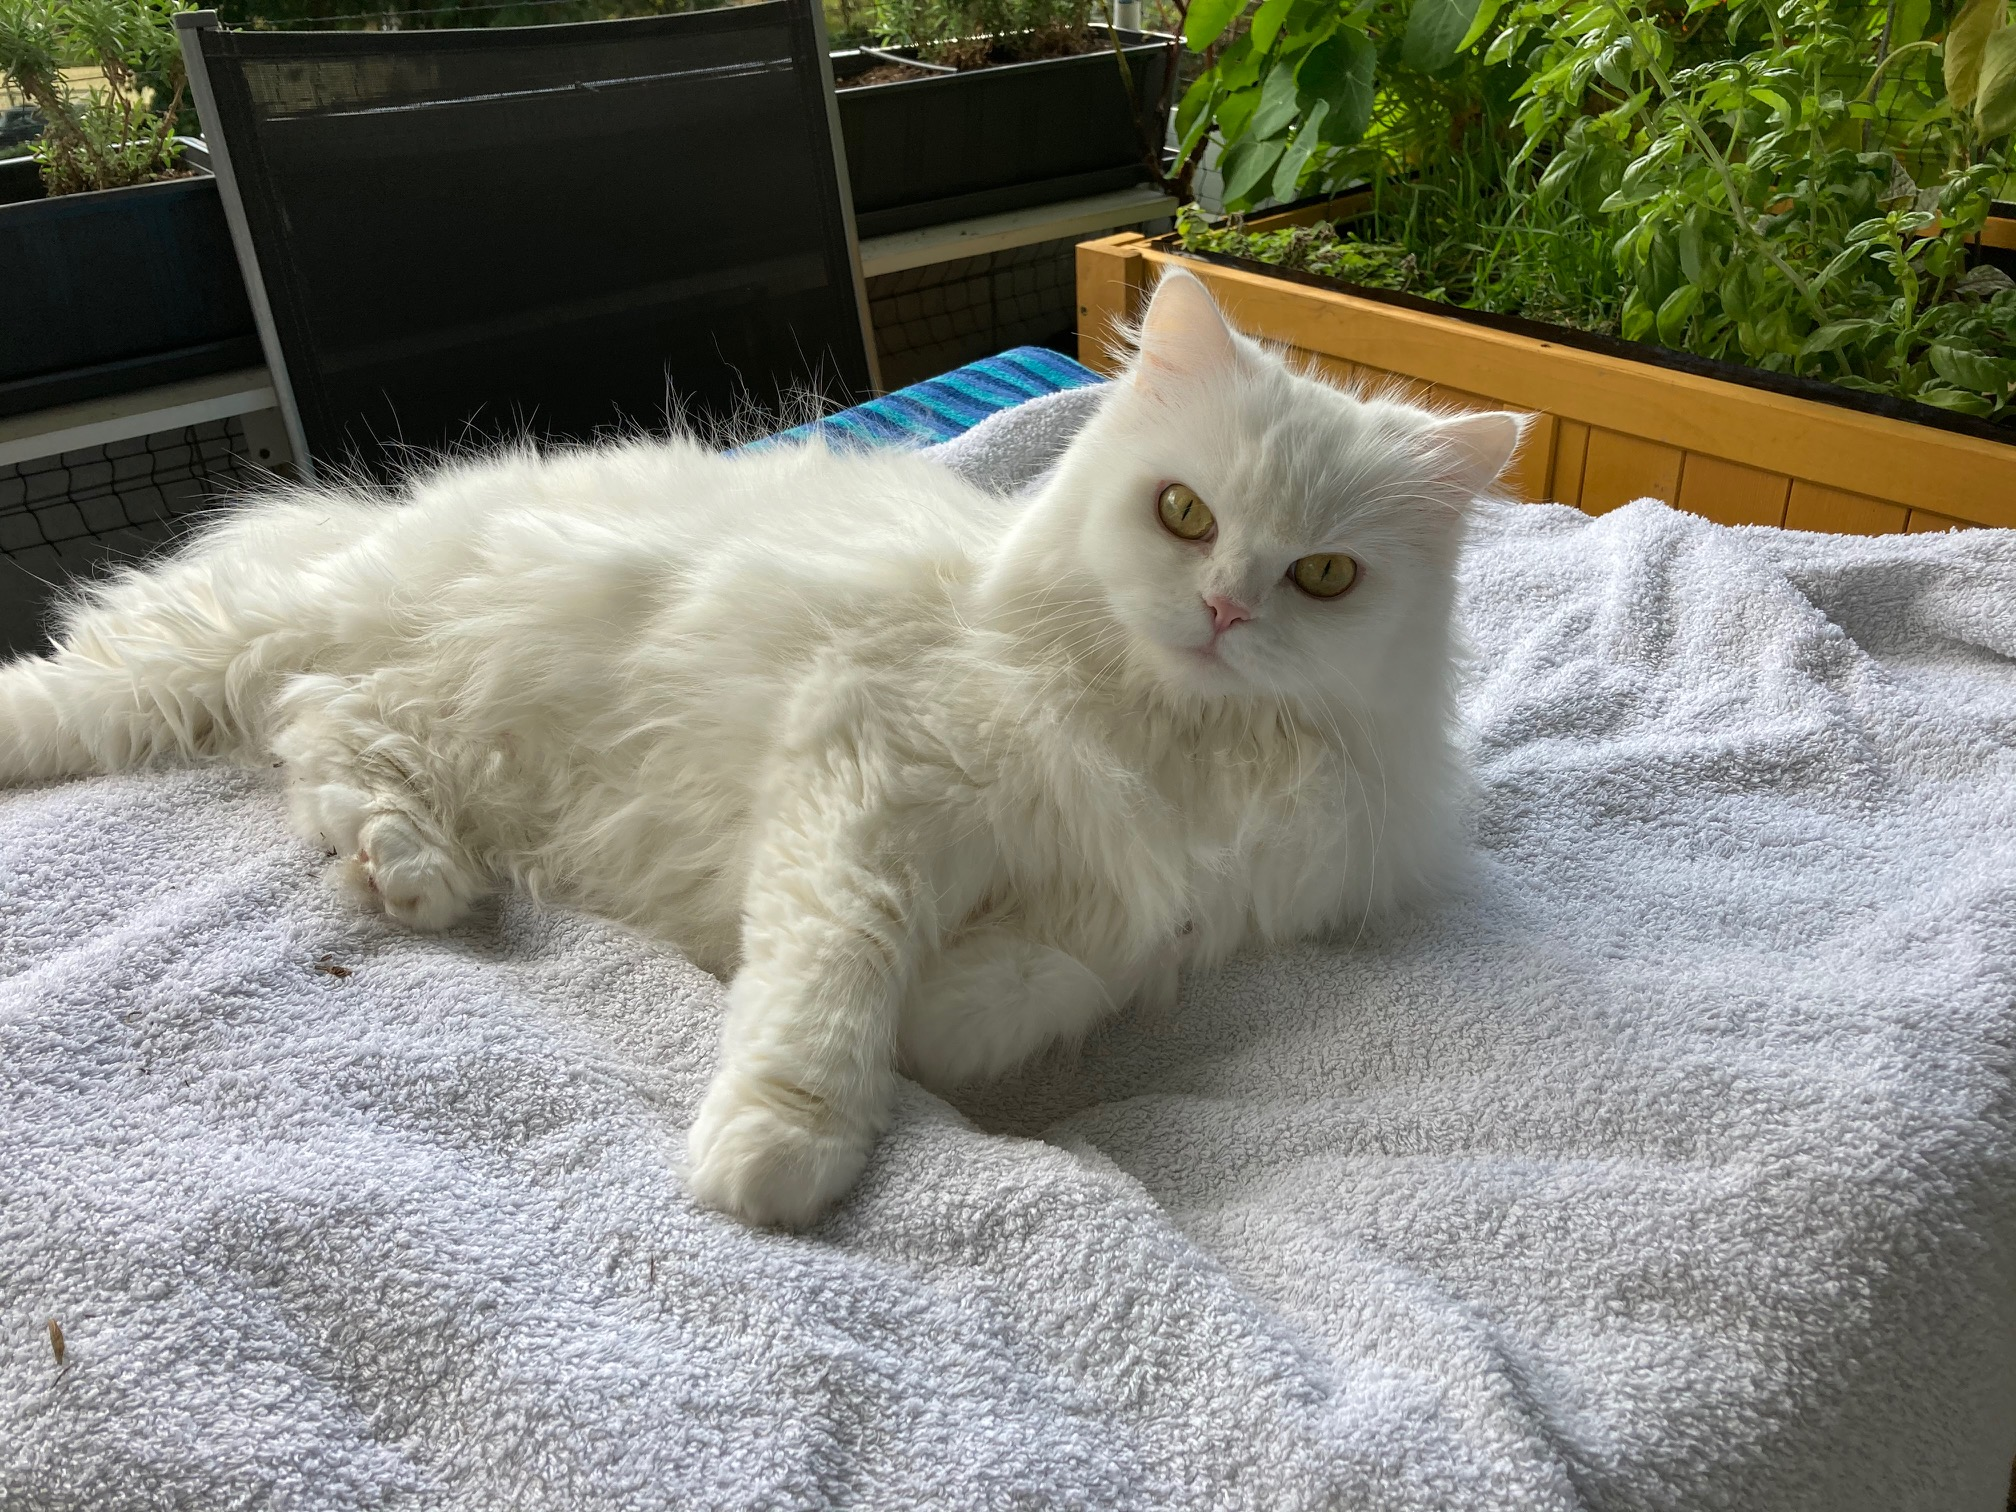
\includegraphics[width=0.5\textwidth]{./Bilder/Katze1.jpg}}
}}
 
 
\AddToShipoutPictureFG{
  \put(100,1100){
\colorbox{gray}{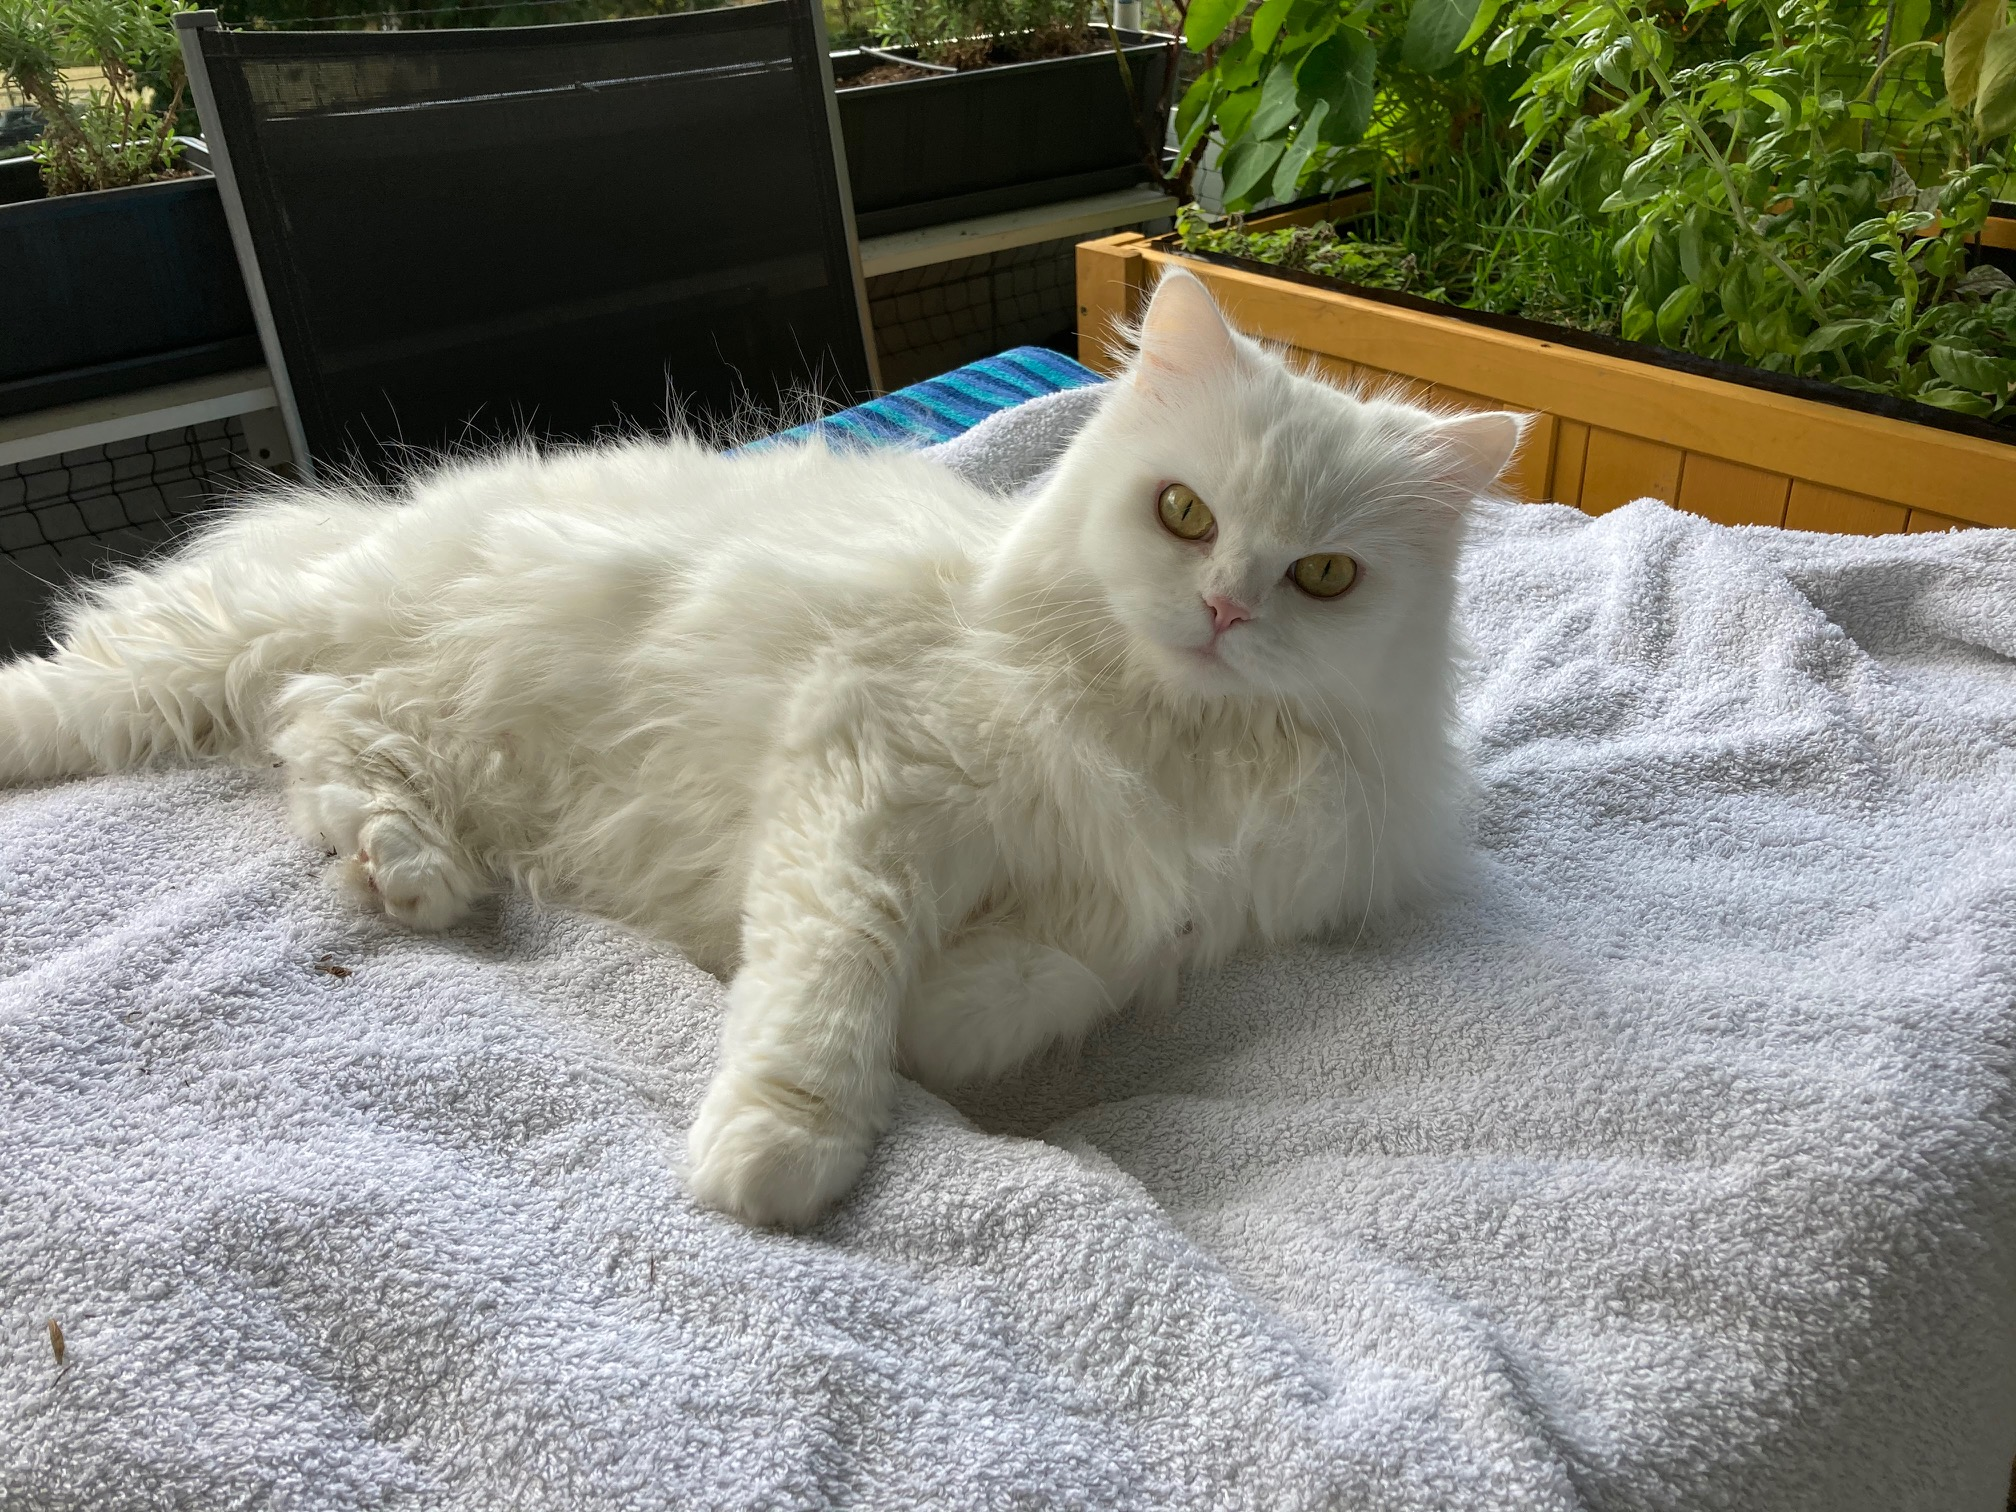
\includegraphics[width=0.5\textwidth]{./Bilder/Katze1.jpg}}
}}
 
 
\AddToShipoutPictureFG{
  \put(1100,750){
\colorbox{gray}{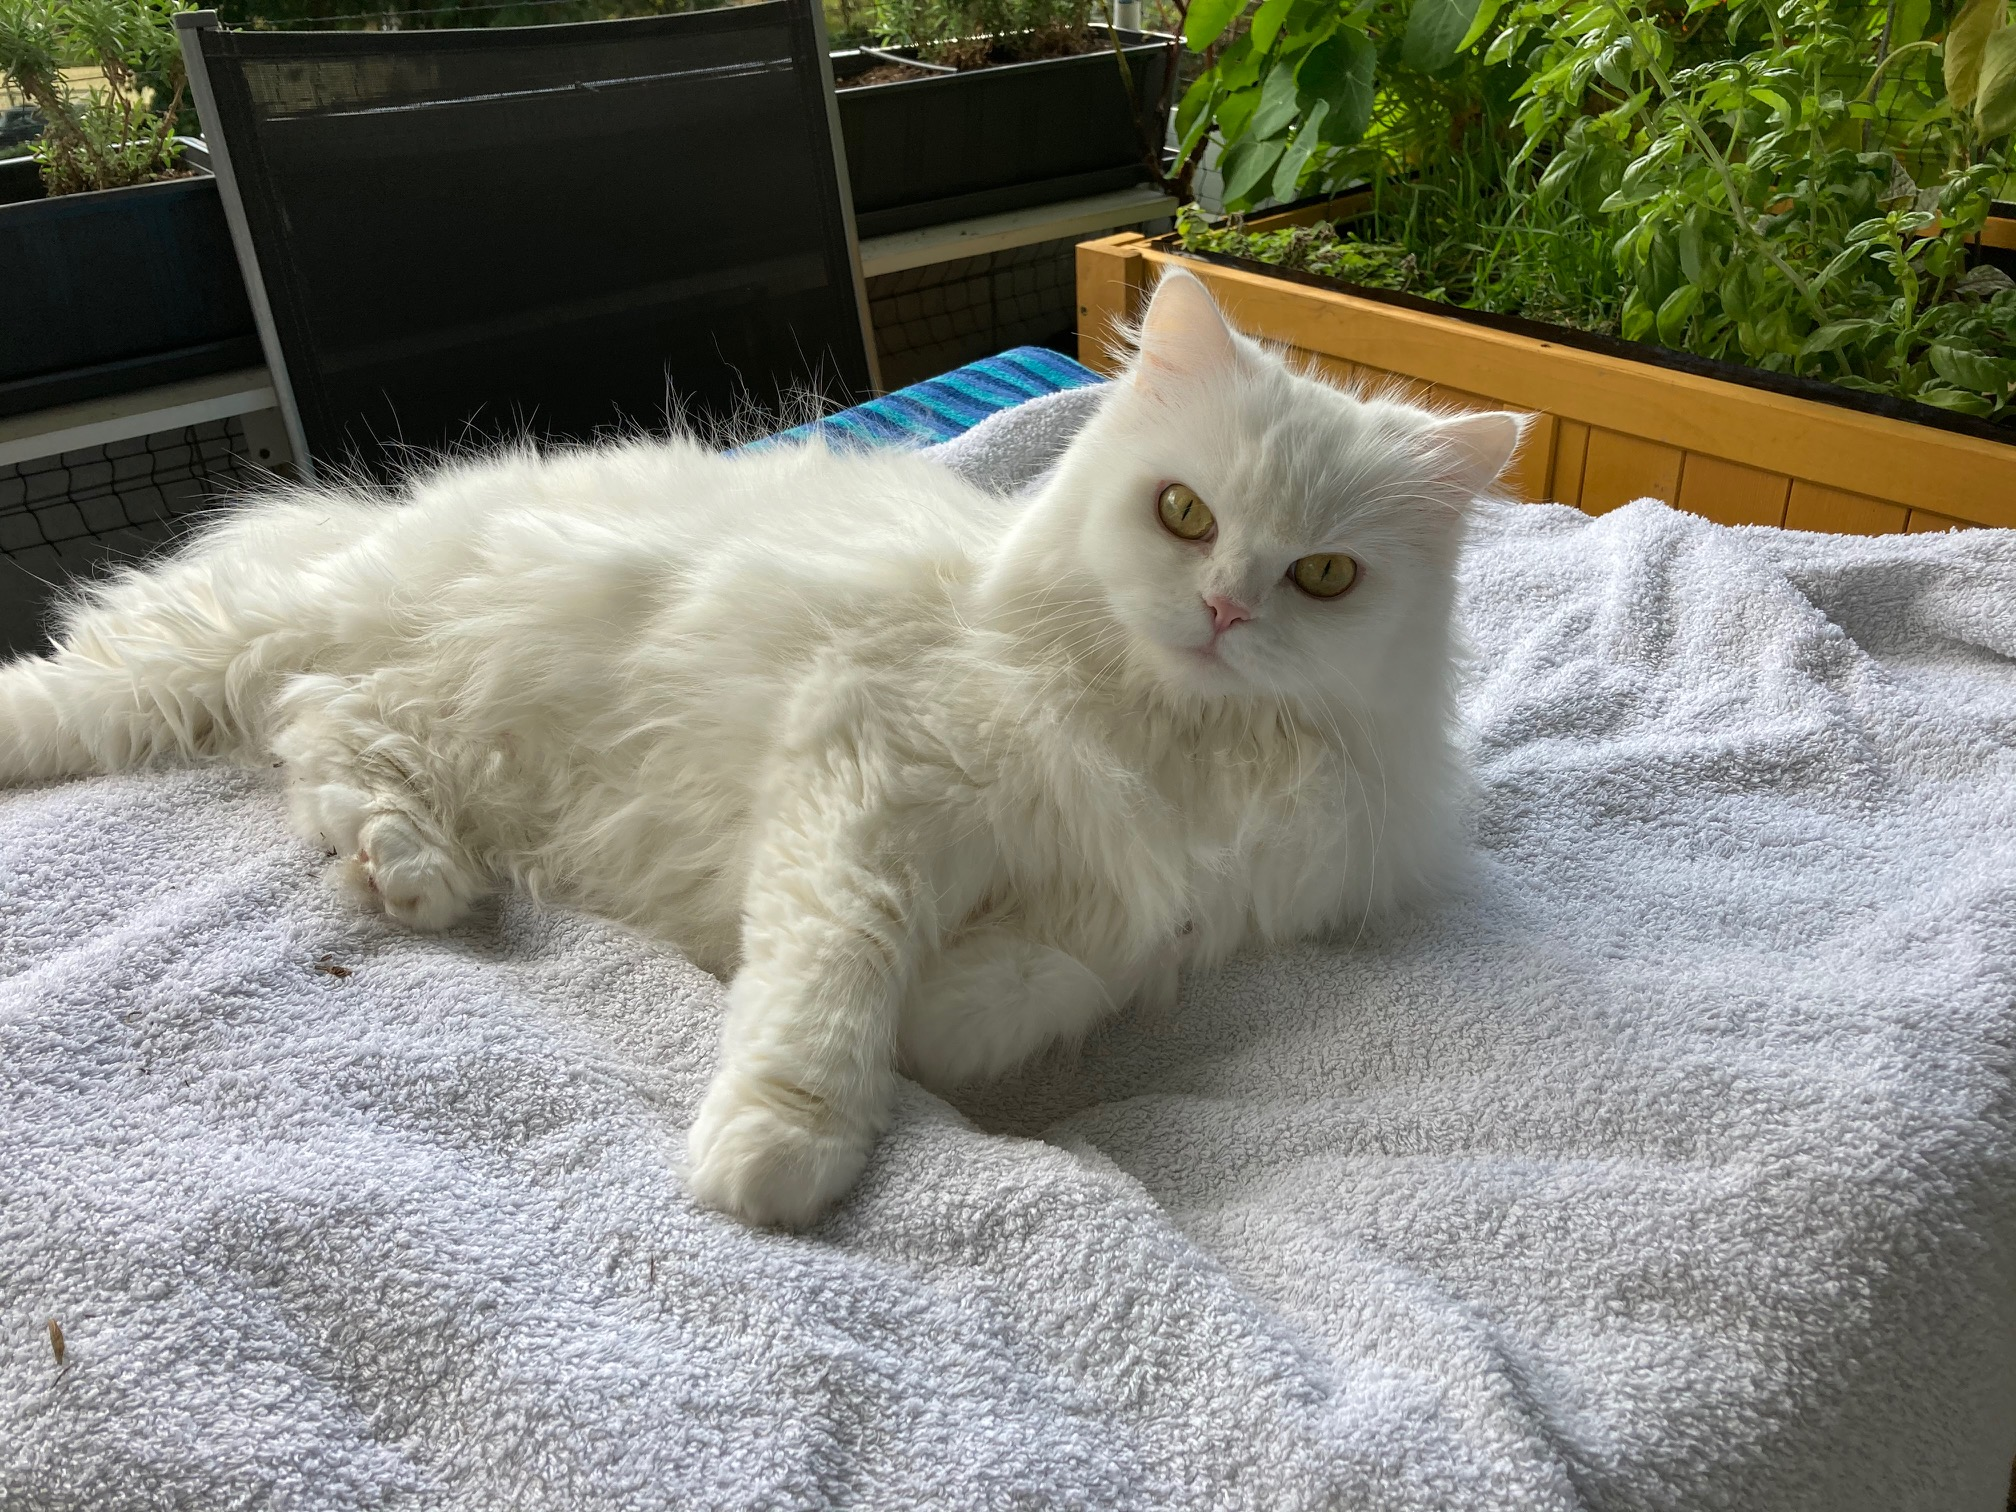
\includegraphics[width=0.5\textwidth]{./Bilder/Katze1.jpg}}
}}